\section{Desarrollo}

\subsection{Fuente $S$}

\par Definiremos una fuente de memoria nula $S$ en base a los frames de capa de enlace capturados. 
La fuente consiste en dos mensajes: un frame fue transmitido de forma \textit{broadcast}, o éste fue transmitido de forma \textit{unicast}.

\subsection{Elección de la fuente $S_1$}

\par Definiremos una fuente de memoria nula $S_1$ en base a las Direcciones IP de los paquetes ARP. 
Deberemos tomar diversas decisiones para definirla correctamente para poder distinguir los nodos apropiados.

\par En primer lugar: debemos elegir si tomar los paquetes \textit{who-has}, \textit{is-at}, o ambos.
En la mayoría de los casos, un \textit{who-has} será respondido por exactamente un \textit{is-at} correspondiente, a menos que el receptor deseado no pueda recibir el paquete o emitir la respuesta, o que haya dos dispositivos con una misma MAC address que intenten responder a la vez.
Por ende, la información del \textit{is-at} será redundante con la del \textit{who-has}, a menos que se produzca un error (lo que, de tomar ambos, agregaría errores a las mediciones).

\par Consecuentemente, tomaremos sólo uno.
Ya que el \textit{who-has} se transmite de forma \textit{broadcast}, mientras que el \textit{is-at}, de forma \textit{unicast}\footnote{Si bien realizaremos las mediciones en modo promiscuo, la presencia de \textit{switches} puede evitar que veamos este tipo de paquetes si no están destinados a nuestro dispositivo, lo que generaría aún más errores en las mediciones.}, tomaremos el primero.

\par En segundo lugar, debemos decidir si emplear el origen del \textit{who-has}, su destino, o ambos como el mensaje de la fuente.
Esta decisión no la tomaremos de antemano, sino que observaremos los grafos resultantes de los experimentos y en base a ellos decidiremos cuál es la opción más acertada.

\par En último lugar, debemos decidir si permitir mensajes repetidos\footnote{Es decir, si considerar repetidas veces múltiples paquetes ARP con igual origen y destino.}. 
Si bien esto no es ilógico desde el punto de vista del modelo de fuente de memoria nula planteado, los paquetes ARP repetidos no deberían ser necesarios: una vez que se envía un \textit{who-has} por una cierta dirección IP y éste es respondido por un \textit{is-at}, la relación entre esta dirección y la MAC address provista debería persistirse en una tabla del emisor; paquetes repetidos podrían ser síntomas de que el \textit{who-has} original no tuvo respuesta, por lo que otros posteriores fueron requeridos.

\par Creemos que por esta razón no deberíamos considerar paquetes repetidos, pero de todas formas juzgaremos ambos procedimientos en base a los resultados de los experimentos.

\par Los grafos que emplearemos para representar la red subyacente de mensajes ARP serán independientes de las elecciones que tomemos respecto de la fuente.
En particular, éstos consistirán en digrafos con loops\footnote{Como mencionamos en la Introducción, en un \textit{gratuitous ARP}, $\text{\textit{Sender's Protocol Address}} = \text{\textit{Target Protocol Address}}$. Para poder observar este fenómeno en el grafo, permitiremos loops.}, donde hay un eje de un nodo a otro si el primero emite un \textit{who-has} preguntando por la Dirección IP del segundo. 

\subsection{Experimento 1: red inalámbrica de los laboratorios del DC}

\par Para este experimento evaluamos la red inalámbrica de los laboratorios del DC.

\subsubsection{Fuente $S$}

\par A continuación podemos ver la fuente $S$ propuesta modelada con los resultados del experimento: \\

\begin{tabular}{ | c | c | c |}
    \hline
    Mensaje & Probabilidad & Información [bits] \\
    \hline
    \textit{Unicast} & 0.773 & 0.371 \\
    \hline
    \textit{Broadcast} & 0.227 & 2.141 \\
    \hline
\end{tabular} \\

\par Entropía de la fuente: 0.772 bits. Entropía máxima: 1 bit.

\par Observamos que la entropía de la fuente es menor que la máxima, ya que las transmisiones \textit{unicast} son casi 3 veces más probables que las \textit{broadcast}.
Esto nos provee una cota inferior para el \textit{overhead} impuesto por los protocolos de control: al menos 22.7\% de los frames no transmiten datos.

\par Ya que no poseemos una idea del comportamiento esperado de esta fuente, no podemos realizar un análisis más detallado sólo a partir de esta fuente.
Por ende, lo profundizaremos recién en la sección del siguiente experimento, comparando con los resultados obtenidos de esa red.
%vemos que la entropía y la probabilidad de los frames \textit{broadcast} son significativamente mayores para la fuente $S$ en el experimento 2.

%\par Podemos ver, comparando la estructura de ambas redes (figuras \ref{ARPDC-sinColapsar} y \ref{ARPTrab-sinColapsar}, respectivamente), que la de este experimento es más fragmentaria, mientras que la del 2 posee un mucho mayor grado de interconexión.

\subsubsection{Fuente $S_1$}

\par En las figuras \ref{ARPDC-sinColapsar} y \ref{ARPDC} se pueden ver los grafos\footnote{Ambos grafos representan la misma red. Sin embargo, el tamaño del grafo \ref{ARPDC-sinColapsar} puede dificultar un análisis detallado, por lo que en la figura \ref{ARPDC} colapsamos ciertos nodos con iguales vecinos (que se muestran en rojo). Mantuvimos el grafo original ya que una mirada rápida ofrece más información concerniente a la topología de la red.} de la red subyacente de mensajes ARP.

\begin{figure*}[ht]
    \centering
    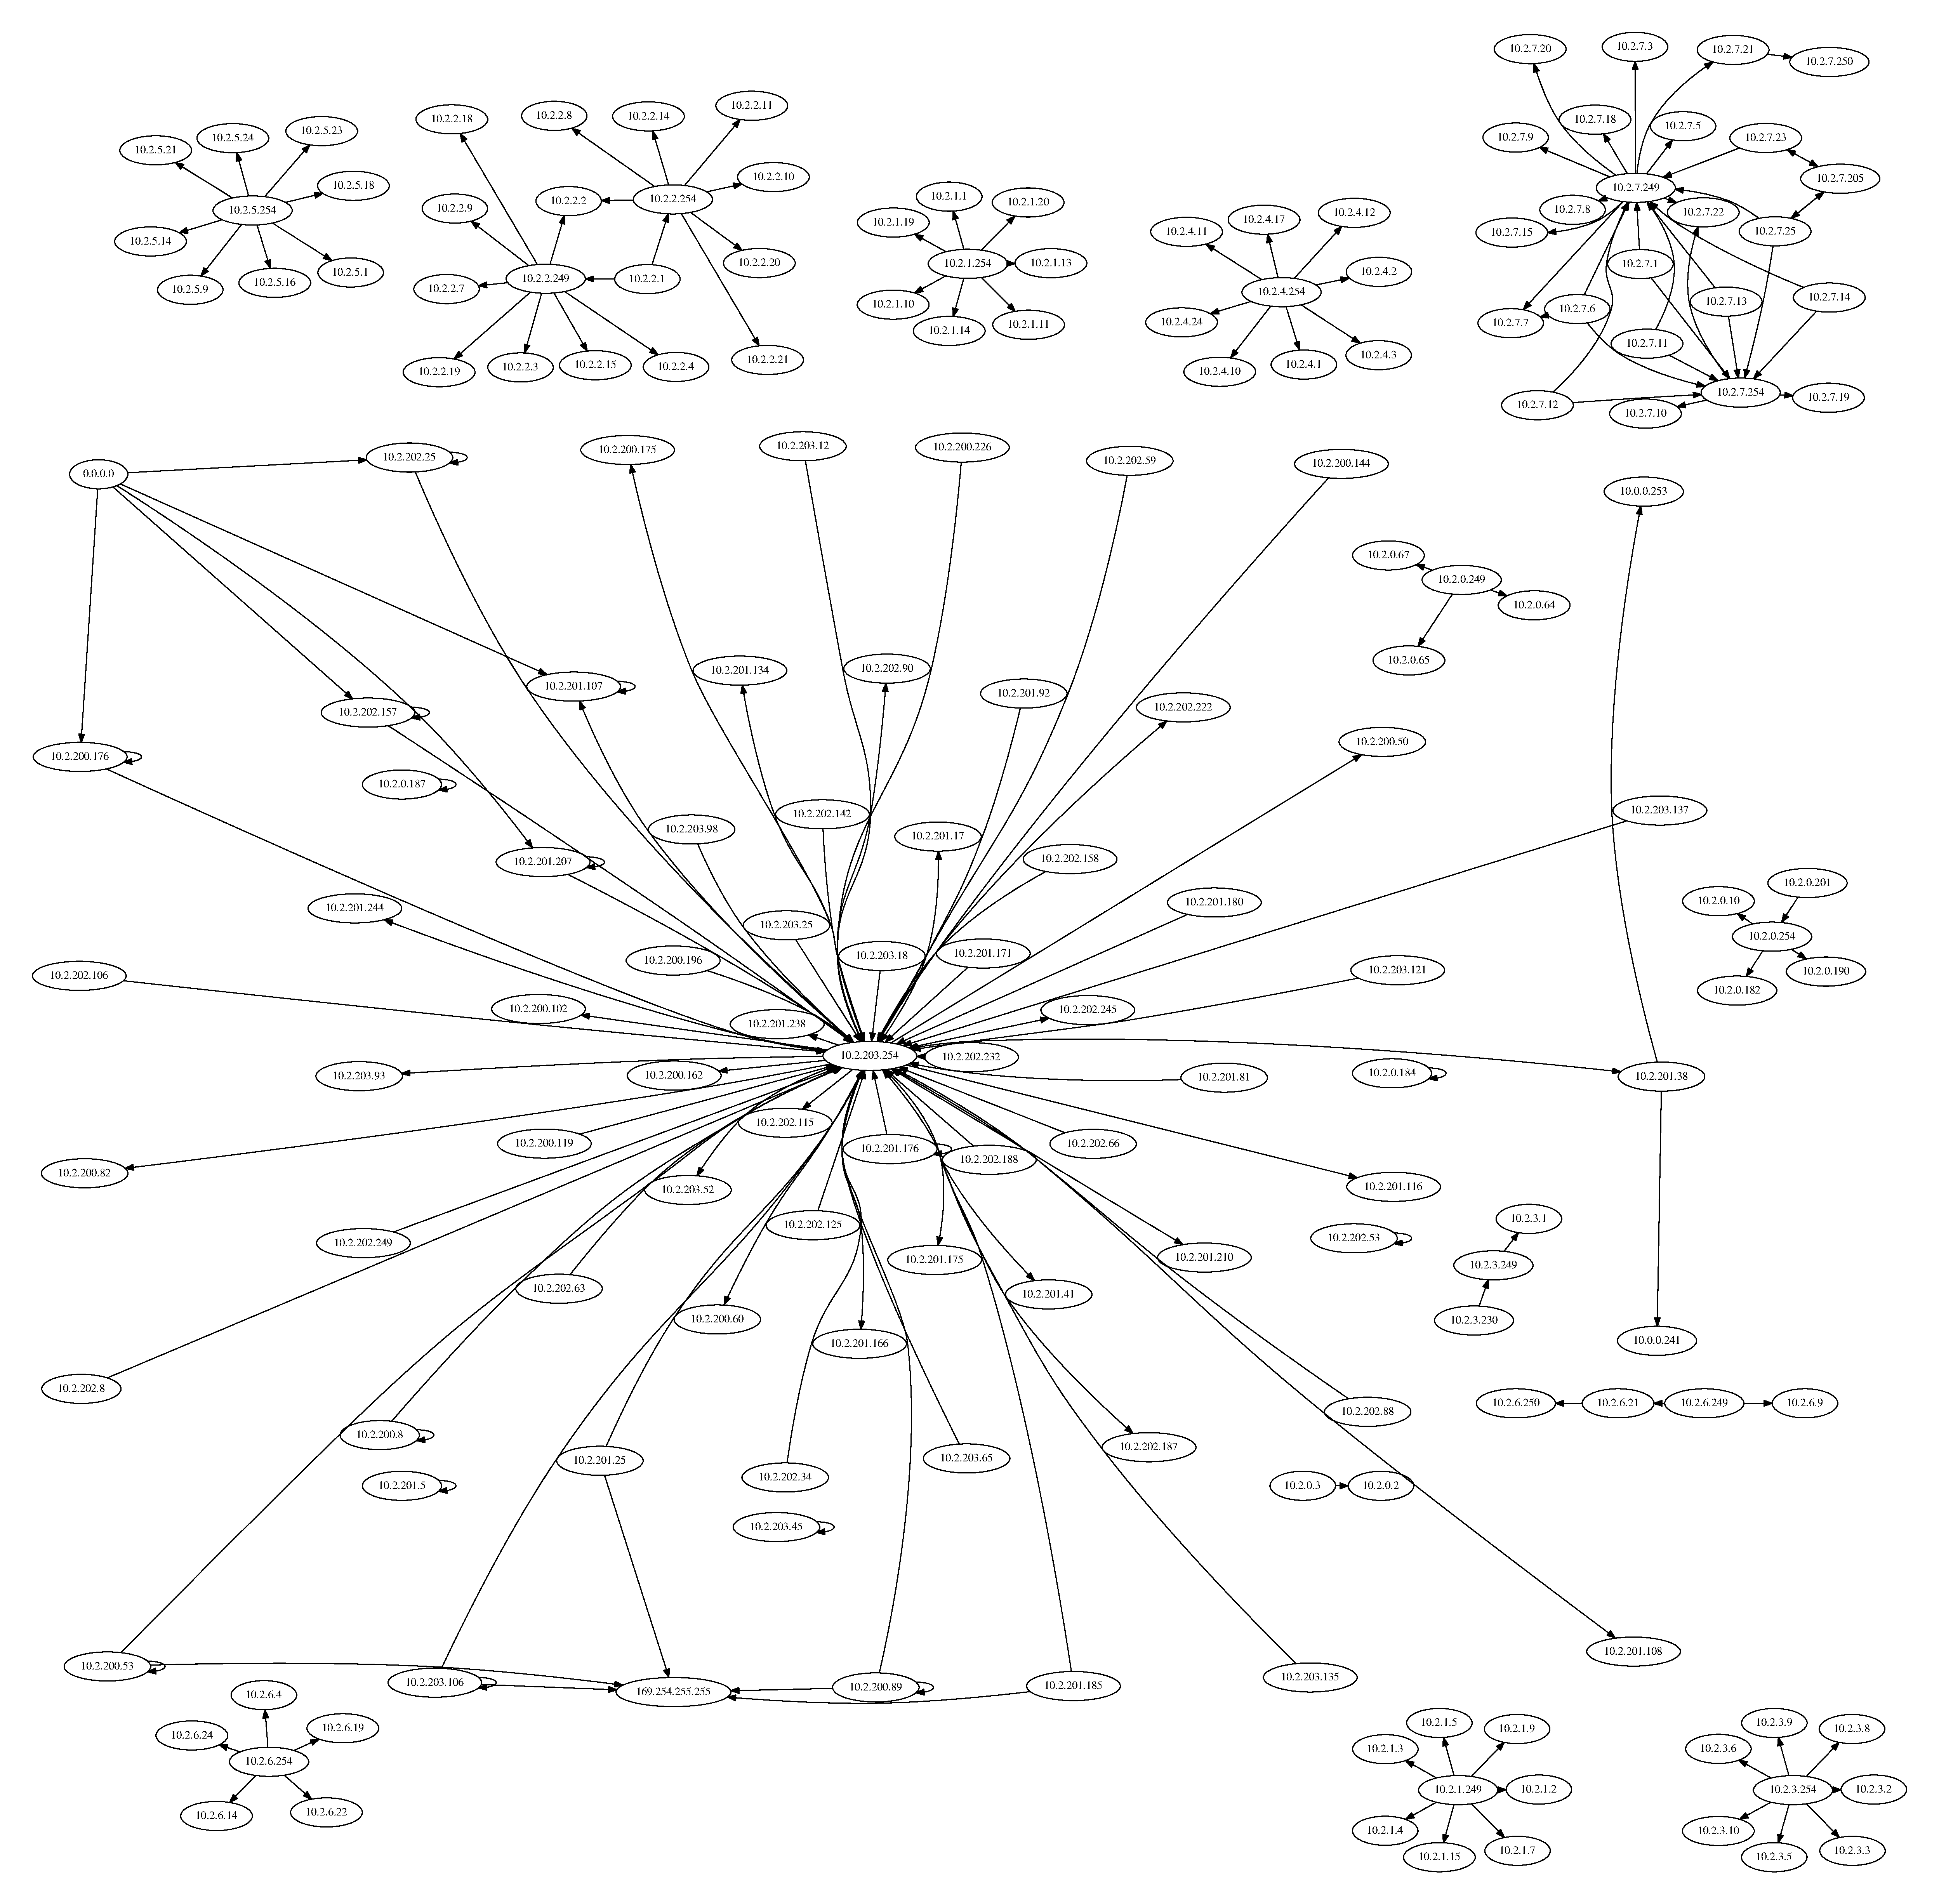
\includegraphics[width=0.9\textwidth]{figuras/ciudad_10_grafoSinColapsar.pdf}
    \caption{Grafo de la red subyacente de mensajes ARP, sin colapsar nodos .}\label{ARPDC-sinColapsar}
\end{figure*}

\begin{figure*}[ht]
    \centering
    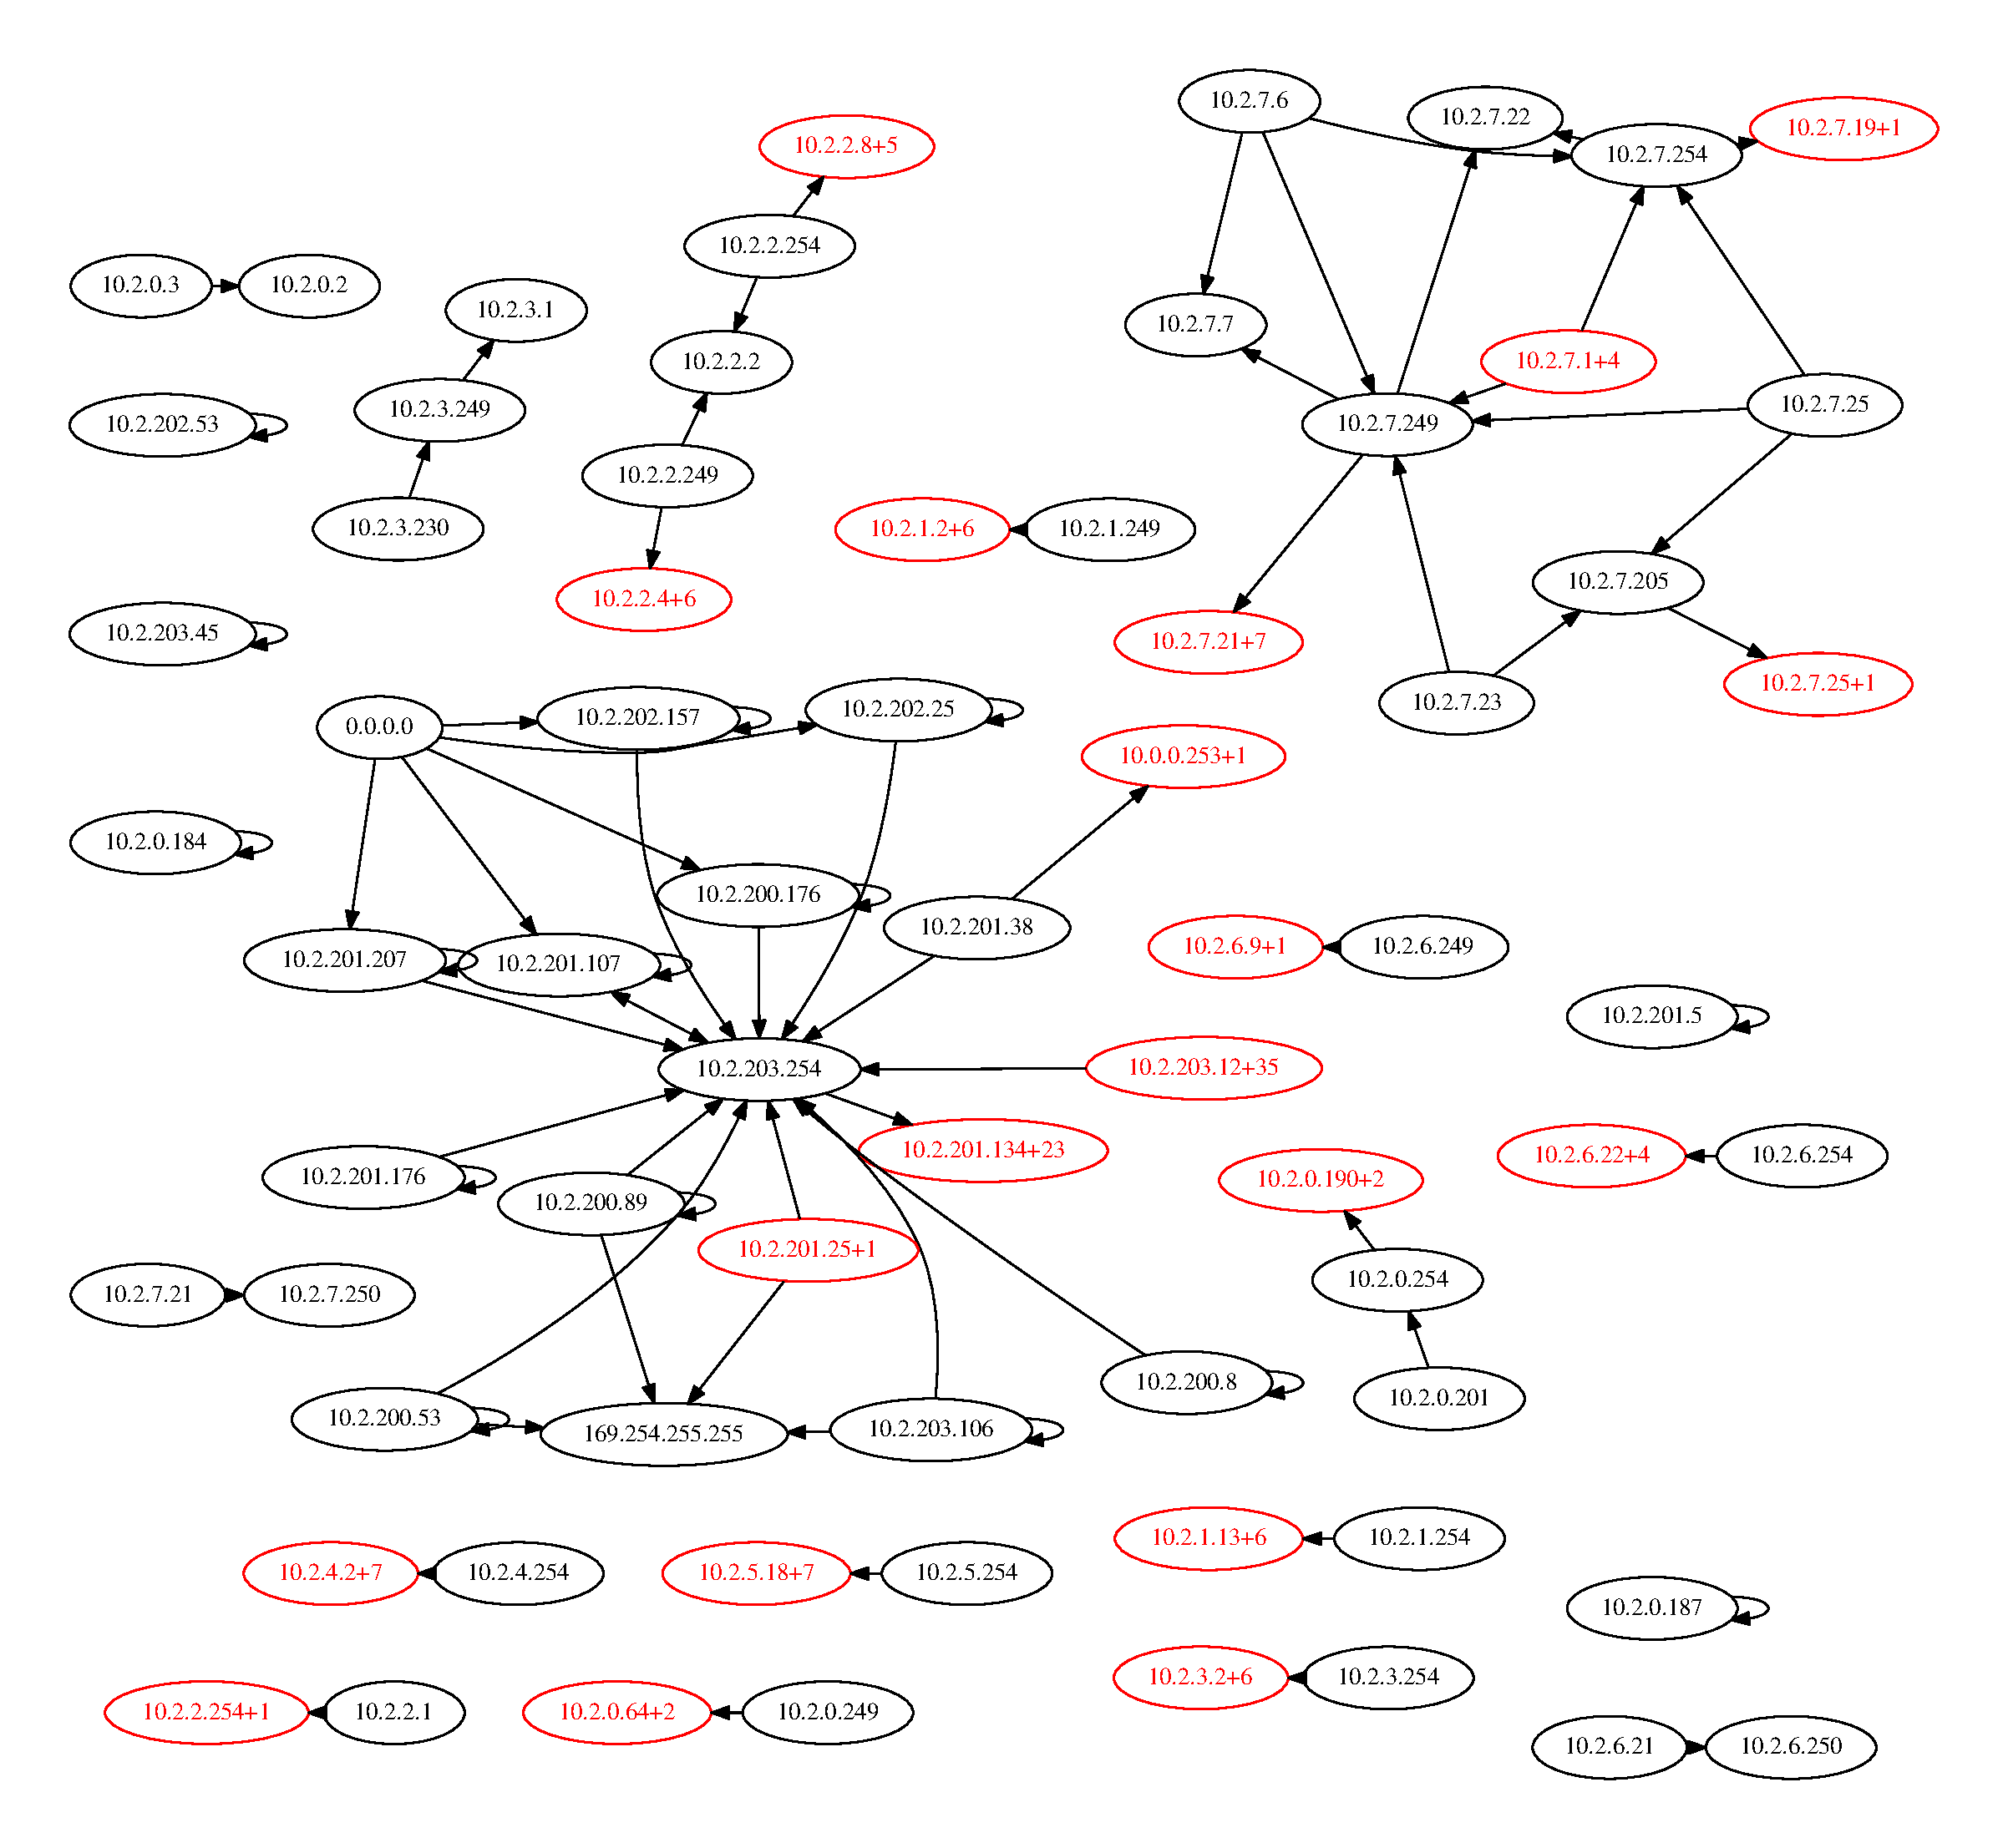
\includegraphics[width=0.9\textwidth]{figuras/ciudad_10_grafo.pdf}
    \caption{Grafo de la red subyacente de mensajes ARP, colapsando nodos.}\label{ARPDC}
\end{figure*}

\par Las direcciones IP de la red son de la forma 10.2.X.Y, con una sola excepción que mencionaremos más adelante.
Éstas son direcciones IP privadas\footnote{Todo el rango 10.0.0.0-10.255.255.255 es privado.}.

\par La red se presenta altamente fragmentada; el grafo posee múltiples componentes conexas.
Adicionalmente, vemos repetido un patrón entre varias de estas componentes: un nodo central, con una dirección IP de la forma 10.2.X.254 o 10.2.X.249, que envía paquetes a múltiples hojas\footnote{Se presenta una estructura de estrella, o cercana.}.
Esta estructura es consistente con el comportamiento esperado de Default Gateways. 

\par Hay un nodo claramente destacado en la red, el de dirección IP 10.2.203.254, que tanto envía como recibe paquetes de un gran número de hojas.

\par Se advierten diversas anomalías: en primer lugar, loops en el grafo, que como mencionamos previamente, se deben a \textit{gratuitous ARPs}; en segundo lugar, la dirección 0.0.0.0 se hace presente en el grafo, siempre como origen, lo que ejemplifica \textit{ARP probing}; finalmente, una única IP que no comienza con 10.2, la 169.254.255.255.
El rango 169.254.0.0-169.254.255.255 está reservado; se asigna cuando un dispositivo no tiene IP estática, y el protocolo dinámico\footnote{DHCP siendo actualmente el más común.} utilizado falla.

\begin{itemize}
	\item Dada la fuente S1, mostrar la cantidad de información de cada símbolo comparando con la entropía de la fuente.
\end{itemize}

Responder las siguientes preguntas (solo dejar las respuestas):

\begin{itemize}
	\item ¿Existe una correspondencia entre lo que se conoce de la red y los nodos distinguidos detectados por la herramienta? ¿Es posible usar el criterio de distinción propuesto como método para descubrir el/los Default Gateway/s de la red? ¿Es preciso?
\end{itemize}

\subsection{Experimento 2}

Descripci\'on del experimiento y de las condiciones del experimento

Incluir por lo menos los siguientes gr\'aficos:

\begin{itemize}
	\item Dada la fuente binaria S, mostrar la cantidad de infomación de cada símbolo comparando con la entropía de la fuente y la entropía máxima
	\item Dados los paquetes ARP, muestre mediante un grafo, la red de mensajes ARP subyacente
	\item Dada la fuente S1, mostrar la cantidad de información de cada símbolo comparando con la entropía de la fuente.
\end{itemize}

Responder las siguientes preguntas (solo dejar las respuestas):

\begin{itemize}
	\item ¿La entropía de la fuente S es máxima? ¿Que sugiere esto acerca de la red? ¿Está relacionado con el overhead impuesto por la red debido a los protocolos de control (i.e.: ARP)?
	\item ¿Cómo es el tráVco ARP en la red? ¿Se pueden distinguir nodos? ¿Cuántos? ¿Indica algo la cantidad? ¿Se les puede adjudicar alguna función especíVca? ¿Hay evidencia parcial que sugiera que algún nodo funciona de forma anómala y/o no esperada?
	\item ¿Existe una correspondencia entre lo que se conoce de la red y los nodos distinguidos detectados por la herramienta? ¿Es posible usar el criterio de distinción propuesto como método para descubrir el/los Default Gateway/s de la red? ¿Es preciso?
\end{itemize}


\subsection{Experimento 3}

Descripci\'on del experimiento y de las condiciones del experimento

Incluir por lo menos los siguientes gr\'aficos:

\begin{itemize}
	\item Dada la fuente binaria S, mostrar la cantidad de infomación de cada símbolo comparando con la entropía de la fuente y la entropía máxima
	\item Dados los paquetes ARP, muestre mediante un grafo, la red de mensajes ARP subyacente
	\item Dada la fuente S1, mostrar la cantidad de información de cada símbolo comparando con la entropía de la fuente.
\end{itemize}

Responder las siguientes preguntas (solo dejar las respuestas):

\begin{itemize}
	\item ¿La entropía de la fuente S es máxima? ¿Que sugiere esto acerca de la red? ¿Está relacionado con el overhead impuesto por la red debido a los protocolos de control (i.e.: ARP)?
	\item ¿Cómo es el tráVco ARP en la red? ¿Se pueden distinguir nodos? ¿Cuántos? ¿Indica algo la cantidad? ¿Se les puede adjudicar alguna función especíVca? ¿Hay evidencia parcial que sugiera que algún nodo funciona de forma anómala y/o no esperada?
	\item ¿Existe una correspondencia entre lo que se conoce de la red y los nodos distinguidos detectados por la herramienta? ¿Es posible usar el criterio de distinción propuesto como método para descubrir el/los Default Gateway/s de la red? ¿Es preciso?
\end{itemize}
